\documentclass[11pt,a4paper]{article}

% ============================================================================
% PACOTES PARA XELATEX / LUALATEX COM SUPORTE UNICODE, TIKZ COLORIDO E TABELAS
% ============================================================================
\usepackage{fontspec}
\usepackage[margin=2.0cm,top=2.2cm,bottom=2.2cm]{geometry}
\usepackage{amsmath,amssymb,amsfonts,amsthm}
\usepackage{mathtools}
\usepackage{xcolor}
\usepackage{graphicx}
\usepackage{booktabs}
\usepackage{longtable}
\usepackage{array}
\usepackage{multirow}
\usepackage{colortbl}
\usepackage{enumitem}
\usepackage{fancyhdr}
\usepackage{titlesec}
\usepackage{tcolorbox}
\tcbuselibrary{skins,breakable,theorems}
\usepackage{tikz}
\usetikzlibrary{arrows.meta,positioning,shapes.geometric,fit,backgrounds,calc,decorations.pathreplacing}
\usepackage{hyperref}

% Configuração de Fontes com Cobertura Ampla de Glifos Unicode
\defaultfontfeatures{Ligatures=TeX}
\IfFontExistsTF{DejaVu Serif}{
  \setmainfont{DejaVu Serif}
  \setsansfont{DejaVu Sans}
  \setmonofont{DejaVu Sans Mono}[Scale=0.86]
}{}

% Paleta de Cores Soberana (Farcaster Purple, Neynar Cyan, Optimism Red, Emerald, Amber)
\definecolor{fcPurple}{HTML}{6A3CFF}
\definecolor{fcDeep}{HTML}{2E1065}
\definecolor{neynarCyan}{HTML}{06B6D4}
\definecolor{neynarDark}{HTML}{083344}
\definecolor{optRed}{HTML}{F43F5E}
\definecolor{emeraldGreen}{HTML}{059669}
\definecolor{amberGold}{HTML}{D97706}
\definecolor{slateBg}{HTML}{F8FAFC}
\definecolor{slateBorder}{HTML}{CBD5E1}
\definecolor{darkInk}{HTML}{0F172A}

\hypersetup{
    colorlinks=true,
    linkcolor=fcPurple,
    citecolor=emeraldGreen,
    urlcolor=neynarCyan,
    pdftitle={Folksonomia Algébrica e Topologia Hipergráfica do Grafo Social Farcaster via API Neynar v2},
    pdfauthor={Arquitetura Soberana Omni Dual-Brain}
}

% Cabeçalho e Rodapé
\pagestyle{fancy}
\fancyhf{}
\fancyhead[L]{\small\textcolor{fcPurple}{\textbf{Folksonomia Algébrica do Grafo Social Farcaster (API Neynar v2)}}}
\fancyhead[R]{\small\textcolor{darkInk}{Omni Dual-Brain Technical Monograph}}
\fancyfoot[C]{\small\thepage}
\renewcommand{\headrulewidth}{0.5pt}

% Traduções e Rótulos Acadêmicos em Português (pt-BR)
\renewcommand{\figurename}{Figura}
\renewcommand{\tablename}{Tabela}
\renewcommand{\refname}{Referências Bibliográficas}

% Caixas para Filosofemas com Rationales e Definições Formais
\newtcolorbox{filosofema}[2][]{
  enhanced,
  breakable,
  colback=slateBg,
  colframe=fcPurple,
  colbacktitle=fcDeep,
  coltitle=white,
  fonttitle=\bfseries\sffamily,
  title={❖ #2},
  arc=3mm,
  boxrule=1.1pt,
  left=4mm,right=4mm,top=3mm,bottom=3mm,
  #1
}

\newtcolorbox{formalismo}[2][]{
  enhanced,
  breakable,
  colback=white,
  colframe=neynarCyan,
  colbacktitle=neynarDark,
  coltitle=white,
  fonttitle=\bfseries\sffamily,
  title={◈ #2},
  arc=2mm,
  boxrule=1.0pt,
  left=4mm,right=4mm,top=3mm,bottom=3mm,
  #1
}

\begin{document}

% ============================================================================
% TÍTULO E RESUMO ACADÊMICO
% ============================================================================
\begin{center}
  {\LARGE\bfseries\color{fcDeep}
  Folksonomia Algébrica e Topologia Hipergráfica do Grafo Social Farcaster:\\[4pt]
  \large Uma Ontologia Operacional Completa sobre o Ecossistema da API Neynar v2}
  \\[12pt]
  {\normalsize\bfseries Núcleo de Engenharia de Protocolos Web3 \& Arquitetura Omni Dual-Brain}\\[2pt]
  {\small\texttt{compilatorum/omni-dual-brain} $\bullet$ Especificação Técnica e Epistemológica em \texttt{pt-BR}}\\[4pt]
  {\footnotesize Data de Publicação: 12 de Novembro de 2026}
\end{center}

\vspace{4pt}
\begin{tcolorbox}[colback=slateBg,colframe=slateBorder,arc=2mm,boxrule=0.8pt]
\textbf{\textcolor{fcDeep}{Resumo}} ---
Este artigo estabelece uma formulação matemática, semiótica e computacional completa para a \textbf{folksonomia emergente do protocolo social descentralizado Farcaster}, instrumentalizada integralmente através da superfície de endpoints da \textbf{API Neynar v2}. Enquanto as folksonomias clássicas da Web 2.0 foram modeladas como hipergrafos tripartitos simples $\mathbb{F} = \langle \mathcal{U}, \mathcal{R}, \mathcal{T}, \mathcal{Y} \rangle$ (usuários, recursos e tags), demonstramos que o Farcaster opera como um \textbf{Hipergrafo Folksonômico Séptuplo Criptograficamente Atestado} $\mathbb{F}_{\text{FC}} = \langle \mathcal{U}_{\text{FID}}, \mathcal{C}_{\text{Cast}}, \mathcal{K}_{\text{Channel}}, \mathcal{A}_{\text{Action}}, \mathcal{F}_{\text{Frame}}, \mathcal{W}_{\text{Wallet}}, \mathcal{Y}_{\text{Neynar}} \rangle$. Formalizamos os invariantes algébricos de propagação de confiança anti-Sybil (\texttt{neynar\_user\_score}), o Laplaciano hipergráfico de co-ocorrência de canais, a entropia de curadoria comunitária e os operadores de tradução determinística para relatórios de impacto on-chain (KarmaHQ). Ademais, catalogamos exaustivamente todos os domínios funcionais da API Neynar v2 (\emph{Users, Casts, Channels, Feeds, Reactions, Notifications, Signers, Frames v2, Webhooks, Storage, Fnames e Moderação}) e enunciamos cinco \textbf{Filosofemas com Rationales} que fundamentam a engenharia do sistema \emph{Omni Dual-Brain}.

\vspace{4pt}
\noindent\textbf{\textcolor{fcDeep}{Palavras-chave:}} Folksonomia Algébrica $\cdot$ Grafo Social Farcaster $\cdot$ API Neynar v2 $\cdot$ Hipergrafos Criptográficos $\cdot$ Resistência Sybil $\cdot$ LangGraph \& MCP.
\end{tcolorbox}

% ============================================================================
% SEÇÃO 1: INTRODUÇÃO E TRANSIÇÃO DA FOLKSONOMIA CLÁSSICA PARA O FARCASTER
% ============================================================================
\section{Da Folksonomia Tripartita Clássica à Hiper-Folksonomia Criptográfica}

O conceito de \emph{folksonomia} (\emph{folk} + \emph{taxonomy}), cunhado originalmente por Thomas Vander Wal \cite{vanderwal2007} e formalizado algebricamente por Peter Mika \cite{mika2005} e Andreas Hotho et al.\ \cite{hotho2006}, descreve sistemas de indexação colaborativa nos quais uma comunidade classifica recursos digitais sem depender de uma hierarquia ontológica centralizada. Na formulação canônica de Hotho et al.\ \cite{hotho2006}, uma folksonomia é uma tupla quaternária:
\begin{equation}
  \mathbb{F}_{\text{clássica}} \triangleq \langle \mathcal{U}, \mathcal{R}, \mathcal{T}, \mathcal{Y} \rangle, \quad \text{onde } \mathcal{Y} \subseteq \mathcal{U} \times \mathcal{R} \times \mathcal{T}
\end{equation}
representa a relação ternária de atribuição (\emph{tag assignment} ou \emph{post}) em que um usuário $u \in \mathcal{U}$ associa uma etiqueta semântica $t \in \mathcal{T}$ a um recurso $r \in \mathcal{R}$.

Contudo, nas redes sociais corporativas da Web 2.0, a relação $\mathcal{Y}$ sofre de três patologias estruturais: (i) \textbf{heteronomia de custódia}, pois o grafo $\mathcal{Y}$ pertence a um servidor privado; (ii) \textbf{vulnerabilidade Sybil}, dado que identidades $u \in \mathcal{U}$ possuem custo marginal zero de falsificação; e (iii) \textbf{passividade semiótica}, visto que os recursos $r \in \mathcal{R}$ são documentos estáticos e não aplicações transacionais.

O protocolo \textbf{Farcaster}, concebido sob o princípio da \emph{Descentralização Suficiente} (\emph{Sufficient Decentralization}) \cite{srinivasan2022farcaster}, resolve essas três patologias ao ancorar a identidade em contratos inteligentes na rede Optimism L2 (\texttt{IdRegistry}, \texttt{KeyRegistry}, \texttt{StorageRegistry}) enquanto propaga mensagens sociais assinadas via chaves Ed25519 em uma malha distribuída de nós (\emph{Hubs / Snapchain}) governada por CRDTs (\emph{Conflict-Free Replicated Data Types}) \cite{shapiro2011crdt}. Sobre essa camada física, a \textbf{API Neynar v2} \cite{neynar2025docs} atua como o indexador hipergráfico universal, enriquecendo os eventos brutos do protocolo com métricas espectrais de qualidade, busca semântica, árvores de conversação, feeds algorítmicos e infraestrutura de \emph{Signers} e \emph{Frames}.

\begin{formalismo}{Definição 1.1 --- Hipergrafo Folksonômico Séptuplo do Farcaster ($\mathbb{F}_{\text{FC}}$)}
Seja o ecossistema Farcaster indexado pela API Neynar v2 representado pela estrutura algébrica séptupla:
\[
  \mathbb{F}_{\text{FC}} \triangleq \big\langle \mathcal{U}_{\text{FID}}, \, \mathcal{C}_{\text{Cast}}, \, \mathcal{K}_{\text{Channel}}, \, \mathcal{A}_{\text{Action}}, \, \mathcal{F}_{\text{Frame}}, \, \mathcal{W}_{\text{Wallet}}, \, \mathcal{Y}_{\text{Neynar}} \big\rangle
\]
onde cada componente satisfaz os seguintes axiomas estruturais (com glifos simbólicos Unicode):
\begin{itemize}[leftmargin=1.4em,itemsep=2pt]
  \item $\forall u \in \mathcal{U}_{\text{FID}} : \text{fid}(u) \in \mathbb{N}^+ \land \exists! \, \omega_{\text{custody}} \in \mathcal{W}_{\text{Wallet}} \text{ tal que } \texttt{IdRegistry}(\text{fid}(u)) = \omega_{\text{custody}}$;
  \item $\forall c \in \mathcal{C}_{\text{Cast}} : \text{hash}(c) \in \mathbb{B}^{20} \ (\texttt{0x}[0\text{--}\text{f}]^{40}) \land \text{Verify}_{\text{Ed25519}}\big(\text{pk}_{\text{signer}}(u), \, \text{hash}(c), \, \sigma(c)\big) = \top$;
  \item $\forall \kappa \in \mathcal{K}_{\text{Channel}} : \kappa = \langle \texttt{id}, \texttt{parent\_url}, u_{\text{lead}}, \mathcal{M}_{\text{mod}}, \mathcal{M}_{\text{member}}, \mathcal{F}_{\text{followers}} \rangle$ define um locus folksonômico temático;
  \item $\forall \alpha \in \mathcal{A}_{\text{Action}} : \alpha \in \{ \texttt{like}\ (\heartsuit), \, \texttt{recast}\ (\circlearrowright), \, \texttt{reply}\ (\hookrightarrow), \, \texttt{quote}\ (\Supset), \, \texttt{follow}\ (\rightharpoonup), \, \texttt{mute}\ (\oslash), \, \texttt{block}\ (\otimes) \}$;
  \item $\forall f \in \mathcal{F}_{\text{Frame}} : f$ é um mini-aplicativo interativo autenticado por pacotes assinados \texttt{FrameActionData};
  \item $\mathcal{Y}_{\text{Neynar}} \subseteq \mathcal{U}_{\text{FID}} \times \mathcal{C}_{\text{Cast}} \times (\mathcal{K}_{\text{Channel}} \cup \{\varnothing\}) \times \mathcal{A}_{\text{Action}} \times (\mathcal{F}_{\text{Frame}} \cup \{\varnothing\}) \times \mathbb{T}$ é o conjunto de hiper-arestas temporais indexadas em tempo real pela API Neynar v2.
\end{itemize}
\end{formalismo}

% ============================================================================
% SEÇÃO 2: DIAGRAMA COLORIDO RENDERIZADO DA TOPOLOGIA HIPERGRÁFICA
% ============================================================================
\section{Topologia Visual do Hipergrafo Folksonômico e do Pipeline Neynar}

A Figura~\ref{fig:hypergraph} ilustra a arquitetura em camadas que conecta o registro on-chain (Optimism L2), o hipergrafo folksonômico tripartito nuclear ($\mathcal{U}_{\text{FID}} \times \mathcal{C}_{\text{Cast}} \times \mathcal{K}_{\text{Channel}}$) e o motor de indexação e escrita da API Neynar v2.

\begin{figure}[htbp]
\centering
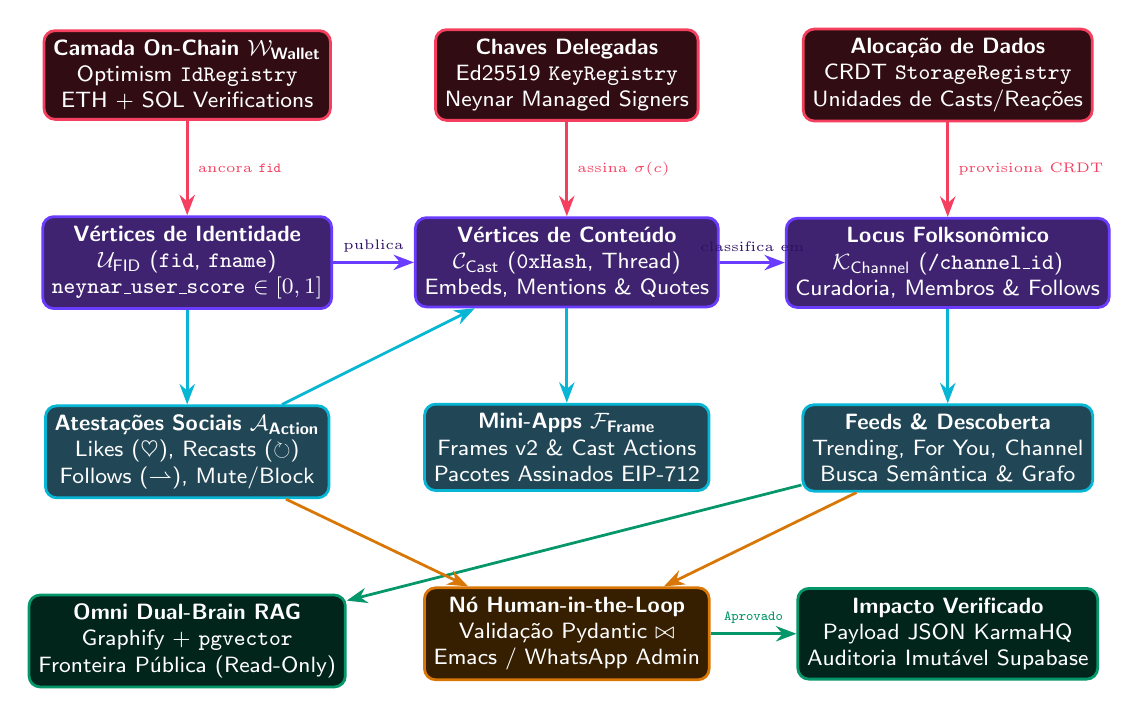
\begin{tikzpicture}[
    node distance=1.0cm and 1.2cm,
    every node/.style={font=\sffamily\footnotesize},
    layerBox/.style={draw, rounded corners=6pt, line width=1.1pt, inner sep=8pt},
    entityPub/.style={draw=neynarCyan, fill=neynarDark!90, text=white, rounded corners=4pt, minimum width=3.1cm, minimum height=1.05cm, align=center, line width=1pt},
    entityFc/.style={draw=fcPurple, fill=fcDeep!92, text=white, rounded corners=4pt, minimum width=3.1cm, minimum height=1.05cm, align=center, line width=1pt},
    entityChain/.style={draw=optRed, fill=optRed!20!black, text=white, rounded corners=4pt, minimum width=3.1cm, minimum height=1.05cm, align=center, line width=1pt},
    entityGreen/.style={draw=emeraldGreen, fill=emeraldGreen!25!black, text=white, rounded corners=4pt, minimum width=3.1cm, minimum height=1.05cm, align=center, line width=1pt},
    entityAmber/.style={draw=amberGold, fill=amberGold!25!black, text=white, rounded corners=4pt, minimum width=3.1cm, minimum height=1.05cm, align=center, line width=1pt},
    arrowStyle/.style={-{Stealth[length=2.6mm]}, line width=1.0pt}
]

% Linha 1: Camada On-Chain & Criptográfica
\node[entityChain] (wallet) {\textbf{Camada On-Chain $\mathcal{W}_{\text{Wallet}}$}\\Optimism \texttt{IdRegistry}\\ETH + SOL Verifications};
\node[entityChain, right=1.3cm of wallet] (signer) {\textbf{Chaves Delegadas}\\Ed25519 \texttt{KeyRegistry}\\Neynar Managed Signers};
\node[entityChain, right=1.3cm of signer] (storage) {\textbf{Alocação de Dados}\\CRDT \texttt{StorageRegistry}\\Unidades de Casts/Reações};

% Linha 2: Hipergrafo Folksonômico Nuclear
\node[entityFc, below=1.2cm of wallet] (ufid) {\textbf{Vértices de Identidade}\\$\mathcal{U}_{\text{FID}}$ (\texttt{fid}, \texttt{fname})\\\texttt{neynar\_user\_score} $\in [0,1]$};
\node[entityFc, below=1.2cm of signer] (ccast) {\textbf{Vértices de Conteúdo}\\$\mathcal{C}_{\text{Cast}}$ (\texttt{0xHash}, Thread)\\Embeds, Mentions \& Quotes};
\node[entityFc, below=1.2cm of storage] (kchan) {\textbf{Locus Folksonômico}\\$\mathcal{K}_{\text{Channel}}$ (\texttt{/channel\_id})\\Curadoria, Membros \& Follows};

% Linha 3: Camada Interativa e Pragmática (Ações e Frames)
\node[entityPub, below=1.2cm of ufid] (actions) {\textbf{Atestações Sociais $\mathcal{A}_{\text{Action}}$}\\Likes ($\heartsuit$), Recasts ($\circlearrowright$)\\Follows ($\rightharpoonup$), Mute/Block};
\node[entityPub, below=1.2cm of ccast] (frames) {\textbf{Mini-Apps $\mathcal{F}_{\text{Frame}}$}\\Frames v2 \& Cast Actions\\Pacotes Assinados EIP-712};
\node[entityPub, below=1.2cm of kchan] (feeds) {\textbf{Feeds \& Descoberta}\\Trending, For You, Channel\\Busca Semântica \& Grafo};

% Linha 4: Orquestração Omni Dual-Brain + Governança HITL
\node[entityGreen, below=1.2cm of actions] (graphify) {\textbf{Omni Dual-Brain RAG}\\Graphify + \texttt{pgvector}\\Fronteira Pública (Read-Only)};
\node[entityAmber, below=1.2cm of frames] (hitl) {\textbf{Nó Human-in-the-Loop}\\Validação Pydantic $\bowtie$\\Emacs / WhatsApp Admin};
\node[entityGreen, below=1.2cm of feeds] (karmahq) {\textbf{Impacto Verificado}\\Payload JSON KarmaHQ\\Auditoria Imutável Supabase};

% Arestas Coloridas
\draw[arrowStyle, optRed] (wallet) -- node[right, font=\tiny, text=optRed] {ancora \texttt{fid}} (ufid);
\draw[arrowStyle, optRed] (signer) -- node[right, font=\tiny, text=optRed] {assina $\sigma(c)$} (ccast);
\draw[arrowStyle, optRed] (storage) -- node[right, font=\tiny, text=optRed] {provisiona CRDT} (kchan);

\draw[arrowStyle, fcPurple] (ufid) -- node[above, font=\tiny, text=fcDeep] {publica} (ccast);
\draw[arrowStyle, fcPurple] (ccast) -- node[above, font=\tiny, text=fcDeep] {classifica em} (kchan);
\draw[arrowStyle, neynarCyan] (ufid) -- (actions);
\draw[arrowStyle, neynarCyan] (actions) -- (ccast);
\draw[arrowStyle, neynarCyan] (ccast) -- (frames);
\draw[arrowStyle, neynarCyan] (kchan) -- (feeds);

\draw[arrowStyle, emeraldGreen] (feeds) -- (graphify);
\draw[arrowStyle, amberGold] (actions) -- (hitl);
\draw[arrowStyle, amberGold] (feeds) -- (hitl);
\draw[arrowStyle, emeraldGreen] (hitl) -- node[above, font=\tiny, text=emeraldGreen] {\texttt{Aprovado}} (karmahq);

\end{tikzpicture}
\caption{Arquitetura em 4 camadas acoplando o Registro On-Chain (Optimism), o Hipergrafo Folksonômico ($\mathcal{U}_{\text{FID}} \times \mathcal{C}_{\text{Cast}} \times \mathcal{K}_{\text{Channel}}$), os indexadores da API Neynar v2 e o Cérebro Único (\emph{Omni Dual-Brain}).}
\label{fig:hypergraph}
\end{figure}

% ============================================================================
% SEÇÃO 3: FORMALISMOS SIMBÓLICOS COM GLIFOS UNICODE
% ============================================================================
\section{Formalismos Simbólicos e Operadores Espectrais da Folksonomia}

\subsection{Tensor de Incidência Folksonômica e Projeções de Co-Ocorrência}

Considere cardinalidades finitas $|\mathcal{U}_{\text{FID}}| = N_u$, $|\mathcal{C}_{\text{Cast}}| = N_c$ e $|\mathcal{K}_{\text{Channel}}| = N_k$. Definimos o \textbf{Tensor de Incidência Folksonômica de 3ª Ordem} $\boldsymbol{\mathcal{T}} \in \mathbb{R}_+^{N_u \times N_c \times N_k}$ cujas entradas ponderam cada publicação e reação social:
\begin{equation}
  \mathcal{T}_{u,c,k} \triangleq \mathbb{I}\big[(u, c, k) \in \mathcal{Y}_{\text{Neynar}}\big] \cdot \left( 1 + \alpha_{\heartsuit} \sum_{v \in \mathcal{L}(c)} \mathcal{Q}_{\text{score}}(v) + \alpha_{\circlearrowright} \sum_{w \in \mathcal{R}(c)} \mathcal{Q}_{\text{score}}(w) \right)
\end{equation}
onde $\mathcal{L}(c) \subseteq \mathcal{U}_{\text{FID}}$ é o conjunto de usuários que atribuíram um \emph{like} ($\heartsuit$) ao cast $c$, $\mathcal{R}(c) \subseteq \mathcal{U}_{\text{FID}}$ é o conjunto de usuários que executaram \emph{recast} ($\circlearrowright$), $\alpha_{\heartsuit} < \alpha_{\circlearrowright}$ são pesos de amplificação social ($\alpha_{\heartsuit}=1, \, \alpha_{\circlearrowright}=2.5$) e $\mathcal{Q}_{\text{score}}(v) \in [0,1]$ é o \texttt{neynar\_user\_score} retornado pela API Neynar v2.

A partir da contração tensorial de $\boldsymbol{\mathcal{T}}$, obtemos três matrizes de adjacência projetadas que governam a semântica emergente da rede \cite{cattuto2007network}:
\begin{align}
  \mathbf{A}^{(\mathcal{K})} &\triangleq \sum_{u \in \mathcal{U}_{\text{FID}}} \sum_{c \in \mathcal{C}_{\text{Cast}}} \mathcal{T}_{u,c,k} \, \mathcal{T}_{u,c,k'} \in \mathbb{R}^{N_k \times N_k} && \text{(Grafo de Afinidade Semântica entre Canais)} \\
  \mathbf{A}^{(\mathcal{U})} &\triangleq \sum_{k \in \mathcal{K}_{\text{Channel}}} \left(\sum_{c} \mathcal{T}_{u,c,k}\right) \left(\sum_{c'} \mathcal{T}_{u',c',k}\right) \in \mathbb{R}^{N_u \times N_u} && \text{(Grafo Homofílico de Comunidade por Canal)} \\
  \mathbf{L}_{\text{norm}}^{(\mathcal{K})} &\triangleq \mathbf{I}_{N_k} - \big(\mathbf{D}^{(\mathcal{K})}\big)^{-1/2} \mathbf{A}^{(\mathcal{K})} \big(\mathbf{D}^{(\mathcal{K})}\big)^{-1/2} && \text{(Laplaciano Normalizado da Folksonomia)}
\end{align}

\subsection{Propagação de Confiança Anti-Sybil (\texttt{neynar\_user\_score}) e Entropia de Canal}

Inspirado no algoritmo \emph{EigenTrust} \cite{kamvar2003eigentrust} e no \emph{PageRank} personalizado \cite{page1999pagerank}, o escore de reputação $\mathcal{Q}_{\text{score}} : \mathcal{U}_{\text{FID}} \to [0,1]$ exposto pela API Neynar v2 nos objetos \texttt{User} (\texttt{experimental.neynar\_user\_score} / \texttt{score}) atenua fazendas de bots através de um ponto fixo contrativo sobre o subgrafo de interações ponderadas $\mathbf{P}$ ancorado em um conjunto semente de \emph{Power Users} verificados $\mathcal{S}_{\text{seed}} \subset \mathcal{U}_{\text{FID}}$:
\begin{equation}
  \vec{q}^{(t+1)} = (1 - \gamma) \, \mathbf{P}^\top \vec{q}^{(t)} + \gamma \, \vec{p}_{\text{seed}}, \quad \text{com } \gamma \in (0, 1) \land \lim_{t \to \infty} \|\vec{q}^{(t+1)} - \vec{q}^{(t)}\|_1 = 0
\end{equation}

Por sua vez, a \textbf{Entropia de Diversidade Comunitária de um Canal} $\kappa \in \mathcal{K}_{\text{Channel}}$ mede se um canal é genuinamente plural ou monopolizado por poucos emissores:
\begin{equation}
  H(\kappa) \triangleq - \sum_{u \in \mathcal{U}(\kappa)} p_\kappa(u) \log_2 p_\kappa(u), \quad \text{onde } p_\kappa(u) = \frac{\sum_{c \in \mathcal{C}(\kappa)} \mathcal{T}_{u,c,\kappa}}{\sum_{v \in \mathcal{U}(\kappa)} \sum_{c \in \mathcal{C}(\kappa)} \mathcal{T}_{v,c,\kappa}}
\end{equation}

% ============================================================================
% SEÇÃO 4: CATÁLOGO COMPLETO DE TODA A API NEYNAR V2 (TABELAS EXAUSTIVAS)
% ============================================================================
\section{Catálogo Sistemático e Taxonômico de Toda a API Neynar v2}

Para que o agente \emph{Omni Dual-Brain} opere sobre a totalidade do grafo social Farcaster, mapeamos nas Tabelas~\ref{tab:neynar_users} a \ref{tab:neynar_actions} todos os subsistemas da API Neynar v2 (\texttt{https://api.neynar.com/v2/farcaster/*}), classificando método HTTP, endpoint, papel folksonômico e formalismo de retorno.

\renewcommand{\arraystretch}{1.22}
\begin{longtable}{@{}p{1.2cm}p{5.2cm}p{4.3cm}p{5.3cm}@{}}
\caption{Domínio I da API Neynar v2 --- Identidade, Usuários, Grafo Social e Reputação ($\mathcal{U}_{\text{FID}}, \mathcal{W}_{\text{Wallet}}$).}\label{tab:neynar_users}\\
\toprule
\rowcolor{fcDeep}
\textcolor{white}{\textbf{Método}} & \textcolor{white}{\textbf{Endpoint Neynar v2}} & \textcolor{white}{\textbf{Papel na Folksonomia}} & \textcolor{white}{\textbf{Operador Simbólico / Campos-Chave}} \\
\midrule
\endfirsthead
\toprule
\rowcolor{fcDeep}
\textcolor{white}{\textbf{Método}} & \textcolor{white}{\textbf{Endpoint Neynar v2}} & \textcolor{white}{\textbf{Papel na Folksonomia}} & \textcolor{white}{\textbf{Operador Simbólico / Campos-Chave}} \\
\midrule
\endhead
\midrule
\multicolumn{4}{r}{\footnotesize\emph{Continua na próxima página...}} \\
\bottomrule
\endfoot
\bottomrule
\endlastfoot
\texttt{GET} & \texttt{/v2/farcaster/user/bulk} & Resolução em lote de perfis por \texttt{fids} e contexto de \texttt{viewer\_fid} & $\Pi_{\mathcal{U}}(F) \to \{\texttt{fid}, \texttt{username}, \texttt{verifications}, \mathcal{Q}_{\text{score}}\}$ \\
\rowcolor{slateBg}
\texttt{GET} & \texttt{/v2/farcaster/user/by\_username} & Resolução canônica de Fname/ENS para identidade $\mathcal{U}_{\text{FID}}$ & $\text{Resolve}(\texttt{fname}) \mapsto u \in \mathcal{U}_{\text{FID}}$ \\
\texttt{GET} & \texttt{/v2/farcaster/user/search} & Busca léxica e ponderada de atores sociais por query $q$ & $\text{Search}_{\mathcal{U}}(q, \texttt{viewer\_fid}) \to \text{Top-}k(\mathcal{U}_{\text{FID}})$ \\
\rowcolor{slateBg}
\texttt{GET} & \texttt{/v2/farcaster/user/bulk-by-address} & Mapeamento reverso On-Chain ($\mathcal{W}_{\text{Wallet}} \to \mathcal{U}_{\text{FID}}$) para ETH e SOL & $\Gamma_{\text{wallet}}^{-1}(\omega_{\text{ETH/SOL}}) \subseteq \mathcal{U}_{\text{FID}}$ \\
\texttt{GET} & \texttt{/v2/farcaster/user/custody-address} & Consulta do endereço de custódia raiz no \texttt{IdRegistry} & $\omega_{\text{custody}}(\text{fid}) \in \mathbb{B}^{20}$ \\
\rowcolor{slateBg}
\texttt{GET} & \texttt{/v2/farcaster/user/power\_lite} & Extração do conjunto semente $\mathcal{S}_{\text{seed}}$ (\emph{Power Badge Users}) & $\mathcal{S}_{\text{seed}} = \{u \in \mathcal{U}_{\text{FID}} \mid \text{power\_badge}(u)=\top\}$ \\
\texttt{GET} & \texttt{/v2/farcaster/followers} & Vizinhança de entrada no dígrafo de interesse ($\text{In-Degree}$) & $\mathcal{N}_{\text{in}}(u) = \{v \in \mathcal{U}_{\text{FID}} \mid v \rightharpoonup u\}$ \\
\rowcolor{slateBg}
\texttt{GET} & \texttt{/v2/farcaster/following} & Vizinhança de saída no dígrafo de interesse ($\text{Out-Degree}$) & $\mathcal{N}_{\text{out}}(u) = \{v \in \mathcal{U}_{\text{FID}} \mid u \rightharpoonup v\}$ \\
\texttt{GET} & \texttt{/v2/farcaster/user/best\_friends} & Subgrafo de afinidade mútua ponderado por frequência de interação & $\text{Affinity}(u,v) = \sum_{\alpha} w_\alpha |\mathcal{A}_{u \leftrightarrow v}^\alpha|$ \\
\rowcolor{slateBg}
\texttt{GET} & \texttt{/v2/farcaster/user/active-channels} & Projeção do usuário sobre os canais onde atua ($\mathcal{U}_{\text{FID}} \to \mathcal{K}_{\text{Channel}}$) & $\text{supp}_{\mathcal{K}}(u) = \{k \in \mathcal{K}_{\text{Channel}} \mid \sum_c \mathcal{T}_{u,c,k} > 0\}$ \\
\end{longtable}

\begin{longtable}{@{}p{1.2cm}p{5.2cm}p{4.3cm}p{5.3cm}@{}}
\caption{Domínio II da API Neynar v2 --- Conteúdo, Árvores Conversacionais e Canais Folksonômicos ($\mathcal{C}_{\text{Cast}}, \mathcal{K}_{\text{Channel}}$).}\label{tab:neynar_casts_channels}\\
\toprule
\rowcolor{neynarDark}
\textcolor{white}{\textbf{Método}} & \textcolor{white}{\textbf{Endpoint Neynar v2}} & \textcolor{white}{\textbf{Papel na Folksonomia}} & \textcolor{white}{\textbf{Operador Simbólico / Campos-Chave}} \\
\midrule
\endfirsthead
\toprule
\rowcolor{neynarDark}
\textcolor{white}{\textbf{Método}} & \textcolor{white}{\textbf{Endpoint Neynar v2}} & \textcolor{white}{\textbf{Papel na Folksonomia}} & \textcolor{white}{\textbf{Operador Simbólico / Campos-Chave}} \\
\midrule
\endhead
\bottomrule
\endlastfoot
\texttt{GET} & \texttt{/v2/farcaster/cast} & Recuperação de cast unitário por \texttt{hash} ou URL Warpcast & $\text{Lookup}_{\mathcal{C}}(h) \to c \in \mathcal{C}_{\text{Cast}}$ \\
\rowcolor{slateBg}
\texttt{GET} & \texttt{/v2/farcaster/casts} & Resolução em lote de múltiplos casts por vetor de hashes & $\Pi_{\mathcal{C}}(H) \subseteq \mathcal{C}_{\text{Cast}}$ \\
\texttt{GET} & \texttt{/v2/farcaster/cast/conversation} & Reconstrução da árvore recursiva de respostas (\emph{Thread DAG}) & $\mathcal{T}_{\text{tree}}(c_{\text{root}}, \text{depth}) = (V_{\text{replies}}, E_{\hookrightarrow})$ \\
\rowcolor{slateBg}
\texttt{GET} & \texttt{/v2/farcaster/cast/search} & Busca full-text e semântica com filtros de autor, canal e data & $\sigma_{q \land \text{channel}=\kappa \land t \in \Delta t}(\mathcal{C}_{\text{Cast}})$ \\
\texttt{POST} & \texttt{/v2/farcaster/cast} & Publicação autenticada de novo Cast, Reply ou Embed via \texttt{signer\_uuid} & $\text{Publish}(\sigma_{\text{signer}}, \text{text}, \kappa, \text{embeds}) \to c^*$ \\
\rowcolor{slateBg}
\texttt{DELETE} & \texttt{/v2/farcaster/cast} & Remoção criptográfica (\emph{Tombstone CRDT}) de cast existente & $\text{RemoveSet}_{\text{CRDT}}(\text{signer\_uuid}, \text{target\_hash})$ \\
\texttt{GET} & \texttt{/v2/farcaster/channel} & Metadados do canal folksonômico, líderes, moderadores e regras & $\kappa = \langle \texttt{id}, u_{\text{lead}}, \mathcal{M}_{\text{mod}}, |\mathcal{F}_{\text{followers}}| \rangle$ \\
\rowcolor{slateBg}
\texttt{GET} & \texttt{/v2/farcaster/channel/search} & Descoberta taxonômica de canais emergentes por domínio & $\text{Search}_{\mathcal{K}}(q) \to \{\kappa_1, \dots, \kappa_m\}$ \\
\texttt{GET} & \texttt{/v2/farcaster/channel/trending} & Ranking de canais por derivada temporal de atividade $\frac{d}{dt}|\mathcal{Y}_\kappa|$ & $\arg\max_{\kappa \in \mathcal{K}} \Delta_{\Delta t}\big(\sum_{u,c} \mathcal{T}_{u,c,\kappa}\big)$ \\
\rowcolor{slateBg}
\texttt{GET} & \texttt{/v2/farcaster/channel/member/list} & Listagem de membros verificados com permissão de postagem no canal & $\mathcal{M}_{\text{member}}(\kappa) \subseteq \mathcal{U}_{\text{FID}}$ \\
\end{longtable}

\begin{longtable}{@{}p{1.2cm}p{5.2cm}p{4.3cm}p{5.3cm}@{}}
\caption{Domínio III da API Neynar v2 --- Feeds, Reações, Signers, Frames v2, Webhooks e On-Chain ($\mathcal{A}_{\text{Action}}, \mathcal{F}_{\text{Frame}}$).}\label{tab:neynar_actions}\\
\toprule
\rowcolor{fcDeep}
\textcolor{white}{\textbf{Método}} & \textcolor{white}{\textbf{Endpoint Neynar v2}} & \textcolor{white}{\textbf{Papel na Folksonomia}} & \textcolor{white}{\textbf{Operador Simbólico / Campos-Chave}} \\
\midrule
\endfirsthead
\toprule
\rowcolor{fcDeep}
\textcolor{white}{\textbf{Método}} & \textcolor{white}{\textbf{Endpoint Neynar v2}} & \textcolor{white}{\textbf{Papel na Folksonomia}} & \textcolor{white}{\textbf{Operador Simbólico / Campos-Chave}} \\
\midrule
\endhead
\bottomrule
\endlastfoot
\texttt{GET} & \texttt{/v2/farcaster/feed/trending} & Feed global ordenado por engajamento ponderado por $\mathcal{Q}_{\text{score}}$ & $\text{Score}(c) = \sum_{v \in \mathcal{L}\cup\mathcal{R}} w_\alpha \mathcal{Q}_{\text{score}}(v) e^{-\lambda \Delta t}$ \\
\rowcolor{slateBg}
\texttt{GET} & \texttt{/v2/farcaster/feed/for\_you} & Recomendação personalizada por difusão no grafo de co-ocorrência & $\vec{r}_u = \mathbf{A}^{(\mathcal{U})} \cdot \mathbf{T}_u$ \\
\texttt{GET} & \texttt{/v2/farcaster/feed/frames} & Subgrafo de casts contendo Mini-Apps / Frames interativos & $\{c \in \mathcal{C}_{\text{Cast}} \mid \text{embeds}(c) \cap \mathcal{F}_{\text{Frame}} \neq \varnothing\}$ \\
\rowcolor{slateBg}
\texttt{POST} & \texttt{/v2/farcaster/reaction} & Emissão de atestação social \texttt{like} ($\heartsuit$) ou \texttt{recast} ($\circlearrowright$) & $\text{React}(\text{signer\_uuid}, \alpha \in \{\heartsuit,\circlearrowright\}, h_{\text{cast}})$ \\
\texttt{GET} & \texttt{/v2/farcaster/reactions/cast} & Auditoria de todos os atores que reagiram a um cast específico & $\mathcal{L}(c) \cup \mathcal{R}(c) \subseteq \mathcal{U}_{\text{FID}} \times \mathbb{T}$ \\
\rowcolor{slateBg}
\texttt{GET} & \texttt{/v2/farcaster/notifications} & Stream de eventos direcionados ao usuário (menções, replies, likes) & $\mathcal{E}_{\text{in}}(u, \text{priority\_mode})$ \\
\texttt{POST} & \texttt{/v2/farcaster/signer} & Criação e registro de par de chaves Ed25519 delegado (\emph{Signer}) & $\text{GenKey}_{\text{Ed25519}}() \to (\text{signer\_uuid}, \text{pk})$ \\
\rowcolor{slateBg}
\texttt{POST} & \texttt{/v2/farcaster/frame/validate} & Validação criptográfica de pacote \texttt{message\_bytes\_in\_hex} de Frame & $\text{Validate}_{\text{Hub}}(\text{packet}) \to \langle u, f, \text{btn\_idx}, \text{tx} \rangle$ \\
\texttt{POST} & \texttt{/v2/farcaster/webhook} & Subscrição reativa em tempo real (\texttt{cast.created}, \texttt{reaction.created}) & $\text{Stream}_{\text{HMAC}}(\text{filters}) \xrightarrow{\text{HTTP POST}} \text{Harness}$ \\
\rowcolor{slateBg}
\texttt{GET} & \texttt{/v2/farcaster/storage/allocations} & Inspeciona capacidade de armazenamento CRDT alugada pelo \texttt{fid} & $\text{Quota}_{\text{CRDT}}(\text{fid}) \to \langle \text{casts}, \text{reactions}, \text{links} \rangle$ \\
\texttt{POST} & \texttt{/v2/farcaster/ban} / \texttt{mute} / \texttt{block} & Operadores de poda defensiva de arestas e moderação de canal & $\mathcal{Y}' = \mathcal{Y} \setminus \{(u_{\text{banned}}, *, \kappa)\}$ \\
\end{longtable}

% ============================================================================
% SEÇÃO 5: DIAGRAMA COLORIDO DE CO-OCORRÊNCIA E IMPACTO KARMAHQ
% ============================================================================
\section{Dinâmica de Co-Ocorrência de Canais e Cruzamento Determinístico Web3}

A Figura~\ref{fig:cooccurrence} apresenta o diagrama colorido do fluxo de agregação espectral pelo qual o subgrafo interno do \emph{Omni Dual-Brain} consome a API Neynar v2 em paralelo à API do GitHub para sintetizar o payload validado pelo Pydantic rumo ao protocolo KarmaHQ.

\begin{figure}[htbp]
\centering
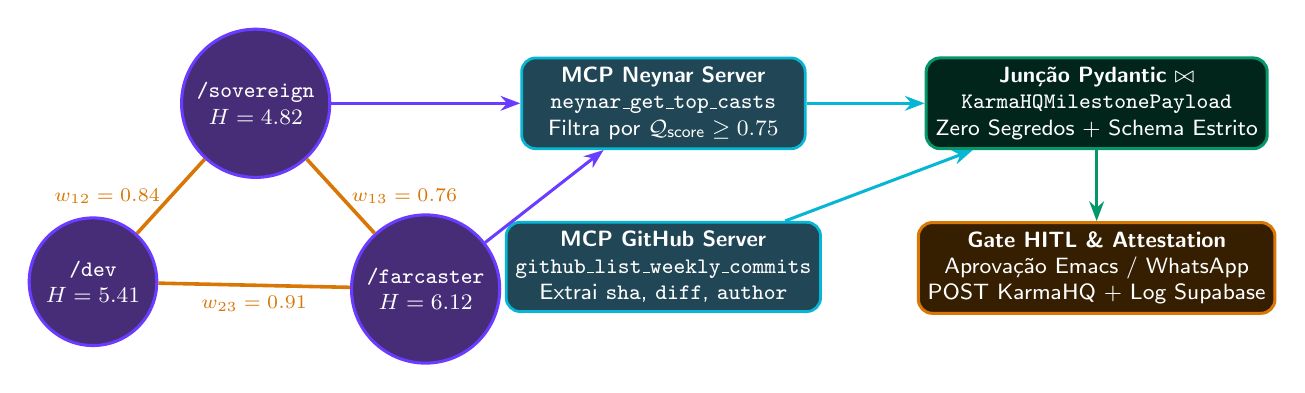
\begin{tikzpicture}[
    node distance=0.9cm and 1.4cm,
    every node/.style={font=\sffamily\footnotesize},
    chanNode/.style={circle, draw=fcPurple, fill=fcDeep!88, text=white, minimum size=1.55cm, align=center, line width=1.1pt},
    procNode/.style={draw=neynarCyan, fill=neynarDark!90, text=white, rounded corners=5pt, minimum width=3.6cm, minimum height=1.1cm, align=center, line width=1pt},
    outNode/.style={draw=emeraldGreen, fill=emeraldGreen!25!black, text=white, rounded corners=5pt, minimum width=3.8cm, minimum height=1.1cm, align=center, line width=1.1pt},
    edgeWeight/.style={line width=1.3pt, color=amberGold}
]

% Subgrafo de Co-Ocorrência de Canais
\node[chanNode] (c1) {\textbf{\texttt{/sovereign}}\\$H=4.82$};
\node[chanNode, below left=1.0cm and 0.8cm of c1] (c2) {\textbf{\texttt{/dev}}\\$H=5.41$};
\node[chanNode, below right=1.0cm and 0.8cm of c1] (c3) {\textbf{\texttt{/farcaster}}\\$H=6.12$};

\draw[edgeWeight] (c1) -- node[left, font=\scriptsize, text=amberGold] {$w_{12}=0.84$} (c2);
\draw[edgeWeight] (c1) -- node[right, font=\scriptsize, text=amberGold] {$w_{13}=0.76$} (c3);
\draw[edgeWeight] (c2) -- node[below, font=\scriptsize, text=amberGold] {$w_{23}=0.91$} (c3);

% Pipeline de Junção Determinística
\node[procNode, right=2.4cm of c1] (neynarMcp) {\textbf{MCP Neynar Server}\\\texttt{neynar\_get\_top\_casts}\\Filtra por $\mathcal{Q}_{\text{score}} \ge 0.75$};
\node[procNode, below=0.9cm of neynarMcp] (githubMcp) {\textbf{MCP GitHub Server}\\\texttt{github\_list\_weekly\_commits}\\Extrai \texttt{sha}, \texttt{diff}, \texttt{author}};

\node[outNode, right=1.5cm of neynarMcp] (pydantic) {\textbf{Junção Pydantic $\bowtie$}\\\texttt{KarmaHQMilestonePayload}\\Zero Segredos + Schema Estrito};
\node[outNode, below=0.9cm of pydantic, draw=amberGold, fill=amberGold!25!black] (hitlGate) {\textbf{Gate HITL \& Attestation}\\Aprovação Emacs / WhatsApp\\POST KarmaHQ + Log Supabase};

\draw[-{Stealth[length=2.5mm]}, line width=1.1pt, fcPurple] (c1) -- (neynarMcp);
\draw[-{Stealth[length=2.5mm]}, line width=1.1pt, fcPurple] (c3) -- (neynarMcp);
\draw[-{Stealth[length=2.5mm]}, line width=1.1pt, neynarCyan] (neynarMcp) -- (pydantic);
\draw[-{Stealth[length=2.5mm]}, line width=1.1pt, neynarCyan] (githubMcp) -- (pydantic);
\draw[-{Stealth[length=2.5mm]}, line width=1.1pt, emeraldGreen] (pydantic) -- (hitlGate);

\end{tikzpicture}
\caption{Projeção do grafo ponderado de co-ocorrência de canais $\mathbf{A}^{(\mathcal{K})}$ acoplado à junção determinística $\mathcal{C}_{\text{GitHub}} \bowtie \mathcal{K}_{\text{Neynar}}$ sob governança Human-in-the-Loop.}
\label{fig:cooccurrence}
\end{figure}

% ============================================================================
% SEÇÃO 6: FILOSOFEMAS COM RATIONALES
% ============================================================================
\section{Filosofemas Arquiteturais e Epistemológicos com Rationales}

Nesta seção enunciamos cinco \textbf{Filosofemas} que sintetizam os princípios primeiros da engenharia do grafo social Farcaster/Neynar e de sua integração no \emph{Omni Dual-Brain}, acompanhados de seus respectivos \textbf{Rationales}.

\begin{filosofema}{Filosofema I --- Soberania do Identificador vs.\ Efemeridade do Cliente}
\emph{``Um grafo social só é epistemologicamente livre quando a identidade do enunciador ($\mathcal{U}_{\text{FID}}$) e a integridade das enunciações ($\mathcal{C}_{\text{Cast}}$) subsistem independentemente da sobrevivência de qualquer interface ou indexador particular.''}

\medskip
\noindent\textbf{Rationale Criptográfico e Arquitetural:}
Nas plataformas monolíticas, o identificador do usuário é uma chave estrangeira aprisionada em um banco relacional privado; se o cliente bani-lo, ele perde simultaneamente seu nome, sua audiência ($\mathcal{N}_{\text{in}}$) e sua memória histórica. No Farcaster \cite{srinivasan2022farcaster}, a separação entre a custódia on-chain do \texttt{fid} (Optimism L2) e os \emph{Signers} delegados Ed25519 permite que múltiplos clientes e agentes autônomos (via API Neynar v2) leiam e escrevam no mesmo hipergrafo sem jamais expor a chave privada raiz de custódia. A interface torna-se substituível; o grafo social permanece inalienável.
\end{filosofema}

\begin{filosofema}{Filosofema II --- Ordem Folksonômica Emergente vs.\ Taxonomia Autoritária}
\emph{``A semântica viva de uma comunidade técnica não pode ser decretada a priori por uma árvore ontológica estática; ela emerge a posteriori como o espectro de autovetores da matriz de co-ocorrência $\mathbf{A}^{(\mathcal{K})}$ entre canais auto-organizados.''}

\medskip
\noindent\textbf{Rationale Topológico e Informacional:}
Conforme demonstrado por Mika \cite{mika2005} e Cattuto et al.\ \cite{cattuto2007network}, taxonomias rígidas envelhecem mais rápido do que a inovação de domínio. No Farcaster, os canais ($\mathcal{K}_{\text{Channel}}$, originalmente ancorados em URLs abertas via FIP-2 e evoluídos para espaços governados por líderes e moderadores) funcionam como bacias de atração semântica. Quando desenvolvedores publicam simultaneamente em \texttt{/dev}, \texttt{/sovereign} e \texttt{/farcaster}, a sobreposição de participantes e reações induz uma métrica riemanniana discreta sobre $\mathcal{K}_{\text{Channel}}$ consultável via \texttt{/v2/farcaster/channel/trending} e \texttt{/v2/farcaster/feed/channels}.
\end{filosofema}

\begin{filosofema}{Filosofema III --- Capital Social Ponderado e Imunidade Anti-Sybil}
\emph{``Em um ambiente onde agentes de IA e scripts automatizados podem gerar milhões de mensagens a custo próximo de zero, a contagem bruta de interações é ruído; somente a interação ponderada pela centralidade espectral de confiança ($\mathcal{Q}_{\text{score}}$) constitui sinal legítimo.''}

\medskip
\noindent\textbf{Rationale Criptoeconômico:}
Qualquer sistema de reputação ou financiamento retroativo de bens públicos (\emph{RetroPGF} / \emph{KarmaHQ}) que utilize cardinalidades ingênuas $|\mathcal{L}(c)|$ incentiva ataques Sybil \cite{kamvar2003eigentrust,buterin2022decentralized}. Ao incorporar o \texttt{neynar\_user\_score} ($\mathcal{Q}_{\text{score}} \in [0,1]$) e os \emph{Power Badges} na função de avaliação $\mathcal{T}_{u,c,k}$, o \emph{Omni Dual-Brain} garante que um único \emph{recast} de um pesquisador ou desenvolvedor central no grafo de confiança tenha peso ordens de grandeza superior a milhares de contas automatizadas periféricas.
\end{filosofema}

\begin{filosofema}{Filosofema IV --- Pragmática Executável (Frames v2 como Atos de Fala Transacionais)}
\emph{``Na teoria dos atos de fala de Austin e Habermas \cite{habermas1981teoria}, dizer algo pode ser fazer algo; no Farcaster, os Frames v2 e Cast Actions convertem o próprio balão conversacional em uma máquina de estados transacional criptograficamente assinada.''}

\medskip
\noindent\textbf{Rationale Semiótico e Computacional:}
Um Cast contendo um \emph{Frame} ($f \in \mathcal{F}_{\text{Frame}}$) deixa de ser texto passivo: quando o usuário clica em um botão, seu cliente assina um pacote \texttt{FrameAction} com sua chave Ed25519 ou dispara uma assinatura EIP-712 da carteira verificada $\omega \in \mathcal{W}_{\text{Wallet}}$. Através do endpoint \texttt{/v2/farcaster/frame/validate} da Neynar, o backend verifica matematicamente quem clicou, em qual cast, dentro de qual canal folksonômico, unificando discurso social e execução financeira/computacional.
\end{filosofema}

\begin{filosofema}{Filosofema V --- A Regra de Ouro da Fronteira Cognitiva Dual (RBAC + HITL)}
\emph{``Um agente conectado simultaneamente ao discurso público e às ferramentas de escrita de protocolo jamais deve possuir autonomia simétrica: a leitura comunitária deve ser livre e sem atrito ($\mathcal{B}_{\text{pub}}$), mas toda mutação de estado ou publicação oficial ($\mathcal{B}_{\text{adm}}$) exige validação estrutural determinística e pausa para deliberação humana ($\mathcal{H}_{\text{HITL}}$).''}

\medskip
\noindent\textbf{Rationale de Segurança de Sistemas Agênticos:}
Dado que o texto proveniente de \texttt{/v2/farcaster/cast/search} ou de webhooks de mensageiros é controlado por terceiros arbitrários, ele constitui um vetor permanente de \emph{Indirect Prompt Injection}. A arquitetura \emph{Omni Dual-Brain} neutraliza esse vetor ao isolar fisicamente as ferramentas MCP por papel (\texttt{role == "public"} vs.\ \texttt{role == "admin"}) e ao exigir que qualquer chamada a \texttt{POST /v2/farcaster/cast} ou submissão ao KarmaHQ passe por um schema Pydantic imutável e aguarde o comando explícito \texttt{"Aprovado"} do administrador no Emacs ou WhatsApp Admin.
\end{filosofema}

% ============================================================================
% SEÇÃO 7: REFERÊNCIAS BIBLIOGRÁFICAS
% ============================================================================
\begin{thebibliography}{99}

\bibitem{vanderwal2007}
Vander Wal, T. (2007).
\emph{Folksonomy Coinage and Definition}.
Off the Top, vanderwal.net. Disponível em: \url{https://vanderwal.net/folksonomy.html}.

\bibitem{mika2005}
Mika, P. (2005).
\emph{Ontologies Are Us: A Unified Model of Social Networks and Semantics}.
In: \textbf{Proceedings of the 4th International Semantic Web Conference (ISWC 2005)}, Lecture Notes in Computer Science, vol.\ 3729, pp.\ 522--536. Springer.

\bibitem{hotho2006}
Hotho, A., Jäschke, R., Schmitz, C., \& Stumme, G. (2006).
\emph{Information Retrieval in Folksonomies: Search and Ranking}.
In: \textbf{The Semantic Web: Research and Applications (ESWC 2006)}, Lecture Notes in Computer Science, vol.\ 4011, pp.\ 411--426. Springer.

\bibitem{cattuto2007network}
Cattuto, C., Schmitz, C., Baldassarri, A., Servedio, V. D. P., Loreto, V., Hotho, A., Grahl, M., \& Stumme, G. (2007).
\emph{Network Properties of Folksonomies}.
\textbf{AI Communications}, 20(4), 245--262.

\bibitem{srinivasan2022farcaster}
Srinivasan, V., \& Romero, D. (2022--2025).
\emph{Farcaster Protocol Architecture: Sufficient Decentralization, Snapchain Consensus, and FIP-2 Channels Specification}.
Merkle Manufactory Technical Documentation. Disponível em: \url{https://docs.farcaster.xyz/}.

\bibitem{neynar2025docs}
Neynar Inc. (2024--2026).
\emph{Neynar v2 API Reference \& OpenAPI Specification: Users, Casts, Channels, Feeds, Frames v2, Signers, and Webhooks}.
Disponível em: \url{https://docs.neynar.com/reference}.

\bibitem{shapiro2011crdt}
Shapiro, M., Preguiça, N., Baquero, C., \& Zawirski, M. (2011).
\emph{Conflict-Free Replicated Data Types}.
In: \textbf{Symposium on Self-Stabilizing Systems (SSS 2011)}, Lecture Notes in Computer Science, vol.\ 6976, pp.\ 386--400. Springer.

\bibitem{kamvar2003eigentrust}
Kamvar, S. D., Schlosser, M. T., \& Garcia-Molina, H. (2003).
\emph{The EigenTrust Algorithm for Reputation Management in P2P Networks}.
In: \textbf{Proceedings of the 12th International Conference on World Wide Web (WWW '03)}, pp.\ 640--651. ACM.

\bibitem{page1999pagerank}
Page, L., Brin, S., Motwani, R., \& Winograd, T. (1999).
\emph{The PageRank Citation Ranking: Bringing Order to the Web}.
Stanford InfoLab Technical Report 1999-66.

\bibitem{buterin2022decentralized}
Weyl, E. G., Ohlhaver, P., \& Buterin, V. (2022).
\emph{Decentralized Society: Finding Web3's Soul}.
\textbf{SSRN Electronic Journal}, Working Paper 4105763.

\bibitem{habermas1981teoria}
Habermas, J. (1981).
\emph{Theorie des kommunikativen Handelns} (\textbf{Teoria do Agir Comunicativo}, Vols.\ 1--2).
Suhrkamp Verlag, Frankfurt am Main.

\end{thebibliography}

\end{document}
